%%%%%%%%%%%%%%%%%%%%%%%%%%%%%%%%%%%%%%%%%%%%%%%%%%%%%%%%%%%%%%%%%%%%%%%%%%%%%%%%
% Preámbulo                                                                    %
%%%%%%%%%%%%%%%%%%%%%%%%%%%%%%%%%%%%%%%%%%%%%%%%%%%%%%%%%%%%%%%%%%%%%%%%%%%%%%%%

\documentclass[11pt,a4paper,titlepage,twoside,openright,openbib]{report}
\usepackage{biblatex}
\usepackage{csquotes}
%%% RELACIÓN DE VARIABLES A PERSONALIZAR %%%
%\def\lingua{gal}
\def\lingua{esp} % descomenta esta liña se redactarás a memoria en español
%\def\lingua{eng} % descomenta esta liña se redactarás a memoria en inglés
\def\nome{Amaro Castro Faci}                             % substitúe aquí o teu nome
\def\nomedirectorA{Outro Nome Completo}             % substitúe aquí o nome de quen dirixe
\def\titulo{Título completo do traballo fin de grao} % substitúe aquí o título do teu TFG  % descomenta a mención correspondente
%\def\mencion{COMPUTACIÓN}
%\def\mencion{ENXEÑARÍA DO SOFTWARE}
%\def\mencion{ENXEÑARÍA DE COMPUTADORES}
%\def\mencion{SISTEMAS DE INFORMACIÓN}
\def\mencion{TECNOLOXÍAS DA INFORMACIÓN}

%\def\renomearcadros{si} % descomenta esta liña se redactas a memoria en español e prefires que
                         % os "cuadros" e o "índice de cuadros" se renomeen
                         % a "tablas" e "índice de tablas" respectivamente

\usepackage{estilo_tfg}

% Lista de paquetes potencialmente interesantes (uso baixo demanda)

% \usepackage{alltt}       % proporciona o entorno alltt, semellante a verbatim pero que respecta comandos
% \usepackage{enumitem}    % permite personalizar os entornos de lista
% \usepackage{eurofont}    % proporciona o comando \euro
% \usepackage{float}       % permite máis opcións para controlar obxectos flotantes (táboas, figuras)
% \usepackage{hhline}      % permie personalizar as liñas horizontais en arrays e táboas
% \usepackage{longtable}   % permite construir táboas que ocupan máis dunha páxina
% \usepackage{lscape}      % permite colocar partes do documento en orientación apaisada
% \usepackage{moreverb}    % permite personalizar o entorno verbatim
% \usepackage{multirow}    % permite crear celdas que ocupan varias filas da mesma táboa
% \usepackage{pdfpages}    % permite insertar ficheiros en PDF no documento
% \usepackage{rotating}    % permite diferentes tipos de rotacións para figuras e táboas
% \usepackage{subcaption}  % permite a inclusión de varias subfiguras nunha figura
% \usepackage{tabu}        % permite táboas flexibles
% \usepackage{tabularx}    % permite táboas con columnas de anchura determinada

%%%%%%%%%%%%%%%%%%%%%%%%%%%%%%%%%%%%%%%%%%%%%%%%%%%%%%%%%%%%%%%%%%%%%%%%%%%%%%%%
% Corpo                                                                        %
%%%%%%%%%%%%%%%%%%%%%%%%%%%%%%%%%%%%%%%%%%%%%%%%%%%%%%%%%%%%%%%%%%%%%%%%%%%%%%%%

\begin{document}

 %%%%%%%%%%%%%%%%%%%%%%%%%%%%%%%%%%%%%%%%
 % Preliminares do documento            %
 %%%%%%%%%%%%%%%%%%%%%%%%%%%%%%%%%%%%%%%%

 \begin{titlepage}
  
  \hspace*{128pt}
  \textcolor{udcpink}{{\fontencoding{T1}\fontfamily{phv}\selectfont Facultade de Informática}}\\[-32pt]

  \begin{center}
    
\includegraphics[scale=0.3]{imaxes/udc}\\[35pt]

    {\large TRABALLO FIN DE GRAO \\
            GRAO EN ENXEÑARÍA INFORMÁTICA \\
            MENCIÓN EN \mencion } \\[100pt]
    
    \begin{huge}
      \begin{spacing}{1.3}
        \bfseries \titulo
      \end{spacing}
    \end{huge}
  \end{center}
  
  \vfill
  
  \begin{flushright}
    {\large
    \begin{tabular}{ll}
      {\bf Estudante:} & \nome \\
      {\bf Dirección:} & \nomedirectorA \\ % COPIA E PEGA ESTA LIÑA MÁIS VECES SE O PRECISAS
    \end{tabular}}
  \end{flushright}
  \rightline{A Coruña, \datasimple\today.}
\end{titlepage}

 \paxinaenbranco
 \dedicatoria{Dedicatoria} % escribe neste comando o teu texto de dedicatoria
 \paxinaenbranco
 \paxinaenbranco
 \begin{agradecementos}
 \blindtext                % substitúe este comando polo teu texto de agradecementos
 \end{agradecementos}
 \paxinaenbranco
 %%%%%%%%%%%%%%%%%%%%%%%%%%%%%%%%%%%%%%%%%%%%%%%%%%%%%%%%%%%%%%%%%%%%%%%%%%%%%%%%

\begin{abstract}\thispagestyle{empty}
  El Cloud Computing es un modelo que permite acceder a un conjunto de recursos, por ejemplo, redes, almacenamiento y cómputo, que pueden ser aprovisionados bajo demanda de forma automatizada y dinámica, reduciendo el coste del servicio para el usuario y el esfuerzo en cuanto a la administración de los recursos. El Centro de Investigación en Tecnoloxías da Información e as Comunicacións (CITIC) de la Universidade da Coruña cuenta con una infraestructura ideada para ofrecer un servicio de Cloud Computing a la comunidad universitaria. Este servicio consiste en que los usuarios pueden aprovisionar un conjunto de recursos del tamaño que requieran para realizar tareas que no serían posibles en dispositivos convencionales. Actualmente ese servicio está activo pero de forma limitada y no abierta a todos los usuarios del CITIC debido a que no existe una plataforma que permita gestionar los perfiles de usuario y su autenticación, ni un portal de acceso para aprovisionar recursos y gestionarlos de forma automatizada. En la actualidad, las tareas de aprovisionamiento y gestión de usuarios se realizan bajo petición previa al administrador del sistema que las ejecuta de forma manual lo cual produce gran coste en tiempo y recursos y aumenta los riesgos del servicio.\\
   El objetivo principal de este proyecto es desplegar un servicio Cloud en el CITIC usando como base las herramientas que ya se encuentran sobre la infraestructura, donde cada usuario pueda tener su un espacio donde gestionar la obtención de recursos y que permita reducir las tareas de administración al integrar el sistema de autenticación de la UDC y al automatizar los procesos de aprovisionamiento, permitiendo establecer unos límites y controlar los recursos que utiliza cada usuario. Todo esto con el fin de mejorar la eficiencia de la infraestructura.\\
   Para evitar problemas en el entorno de producción, el proyecto se desarrollará en un entorno de pruebas para mostrar las funcionalidades y características de la solución implementada pero que tendrán menor rendimiento que el entorno real por contar con recursos reducidos. El proceso se realizará siguiendo la metodología incremental Scrum en la cual primero se analizarán las diferentes alternativas disponibles y posteriormente se irán desplegando componentes para añadir nuevas funcionalidades que completen los objetivos del proyecto.
    % El Cloud Computing es un modelo que permite acceder a un conjunto de recursos, como por ejemplo, redes, almacenamiento, aplicaciones, servicios y potencia de cálculo, que pueden ser aprovisionados bajo demanda de una forma rápida sencilla, reduciendo el coste del servicio para el usuario y el esfuerzo en cuanto a gestión de los recursos.\\
  %  El Centro de Investigación en Tecnoloxías da Información e as Comunicacións (CITIC) de la Universidade da Coruña cuenta con una infraestructura ideada para ofrecer un servicio de Cloud Computing a la comunidad universitaria. Este servicio consiste en que los usuarios pueden aprovisionar un conjunto de recursos, que se traducen en máquinas virtuales, del tamaño que necesiten para realizar tareas que no serían posibles en dispositivos convencionales.\\
    % Actualmente el servicio está activo pero de forma limitada y no abierta a todos los usuarios del CITIC debido que no existe una plataforma que habilite el acceso a cada usuario a sus recursos, que gestione la autenticación de los usuarios, y que automatice y simplifique los procesos de aprovisionamiento de recursos. Hasta ahora, las tareas de aprovisionamiento y gestión de usuarios se realizan bajo petición previa al administrador del sistema y se ejecutan de forma manual lo cual consume más tiempo, recursos, y aumenta los riesgos sobre el servicio.\\
    % El objetivo principal de este proyecto es desplegar un servicio Cloud en el CITIC usando como base las herramientas que ya se encuentran sobre la infraestructura, donde cada usuario pueda tener su propio espacio donde poder gestionar sus recursos según sus necesidades y de forma simple y dinámica, que simplifique la gestión de usuarios integrando el sistema de autenticación de la UDC en el servicio, y establecer un sistema de valoración de los recursos para poder controlar y limitar la cantidad de recursos que un usuario puede aprovisionar para mejorar el uso y funcionamiento del servicio. En definitiva, el objetivo es desplegar un entorno Cloud que haga la infraestructura física más eficiente y para entregar todo su potencial.
  \vspace*{20pt}
\begin{multicols}{2}
\begin{description}
\item [\palabraschaveprincipal:] \mbox{} \\[-20pt]
  \blindlist{itemize}[7] % substitúe este comando por un itemize
                         % que relacione as palabras chave
                         % que mellor identifiquen o teu TFG
                         % no idioma principal da memoria (tipicamente: galego)
\end{description}
\begin{description}
\item [\palabraschavesecundaria:] \mbox{} \\[-20pt]
  \blindlist{itemize}[7] % substitúe este comando por un itemize
                         % que relacione as palabras chave
                         % que mellor identifiquen o teu TFG
                         % no idioma secundario da memoria (tipicamente: inglés)
\end{description}
\end{multicols}

\end{abstract}

%%%%%%%%%%%%%%%%%%%%%%%%%%%%%%%%%%%%%%%%%%%%%%%%%%%%%%%%%%%%%%%%%%%%%%%%%%%%%%%%

 \paxinaenbranco

 \pagenumbering{roman}
 \setcounter{page}{1}

 \tableofcontents
 \listoffigures
 \listoftables
 \cleardoublepage
 
 \pagenumbering{arabic}
 \setcounter{page}{1}
 \bstctlcite{IEEEexample:BSTcontrol}

 %%%%%%%%%%%%%%%%%%%%%%%%%%%%%%%%%%%%%%%%
 % Capítulos                            %
 %%%%%%%%%%%%%%%%%%%%%%%%%%%%%%%%%%%%%%%%

 \chapter{Introdución}
\label{chap:introducion}

\lettrine{P}{rimer} capítulo da memoria, onde xeralmente se exporán as
liñas mestras do traballo, os obxectivos, etc. Incluimos un par de
exemplos de citas~\cite{ErlangBook,ErlangWebBook} e de referencias
internas (sección \ref{sec:mostra}, páxina \pageref{sec:mostra}).

\Blindtext

\section{Sección de mostra}
\label{sec:mostra}

\Blindtext

\subsection{Subsección de mostra}

\Blindtext

 \chapter{Estado de los recursos}
\label{chap:estadoInfraestructuraSistema}
\lettrine{C}{on} el fin de contextualizar los recursos que se utilizarán en este trabajo, en este capítulo se expone la situación actual de toda la infraestructura en lo relacionado al software que está en funcionamiento, a los recursos físicos de los que se compone, y al estado actual de las herramientas que rodean a dichos recursos.

\section{Infraestructura}
La infraestructura física de este servicio de virtualización, se encuentra localizada en el edificio del CITIC de la UDC, dentro de un rack alojado en su Centro de Proceso de Datos (CPD) \cite{citicUDC}. Está formado por 5 nodos \textit{Lenovo NeXtScale nx360 M5} y 3 nodos \textit{Dell EMC PowerEdge R740}. Ambos componentes dan flexibilidad en cuanto a la escalabilidad y ofrecen gran rendimiento de cómputo.\\

Especificaciones principales de los nodos:
\begin{itemize}
    \item Lenovo NeXtScale nx360 M5: 
        \begin{itemize}
            \item CPU: Dos Intel Xeon E5-2650
            \item Memoria: 128 GB
            \item Tarjeta  gráfica: Tesla M60
        \end{itemize}
            Más información: \url{https://lenovopress.com/tips1195-nextscale-nx360-m5-e5-2600-v3}
    \item Dell EMC PowerEdge R740:
        \begin{itemize}
            \item CPU: Dos Xeon Gold 6146
            \item Memoria: 384 GB
            \item Tarjeta gráfica: Tesla P40
        \end{itemize}
    Más información: \url{https://www.dell.com/es-es/work/shop/servidores-almacenamiento-y-redes/smart-value-poweredge-r740-server-standard/spd/poweredge-r740/per7400m}
\end{itemize}
El almacenamiento está colocado físicamente en la misma ubicación que los hosts pero en su abstracción lógica este es independiente y está separado de cada nodo. Está conformado por 13 discos duros SSD de 3.84 TB de capacidad, obteniendo así una capacidad total de casi 50 TB, pero que utilizan la configuración de almacenamiento RAID 5[Pal. \ref{itm:raid5}] lo cual permite conseguir mayor  integridad de los datos, tolerancia a fallos y ancho de banda, reduciendo la cantidad de almacenamiento utilizable a 34 TB. Estos discos forman un \textit{pool} de almacenamiento que se divide en cinco LUNs (\textit{Logical Storage Unit})[Pal. \ref{itm:lun}] de 2 TB cada una, representadas en el sistema de virtualización como cinco \textit{datastores} diferentes que utilizan el sistema de archivos VMFS el cual optimiza el almacenamiento de máquinas virtuales.\\
Los discos duros físicos están colocados en una misma cabina y son accesibles por todos los nodos a través de dos switches para aportar redundancia. Para ello, las cabinas incorporan dos controladores con conexión SFP+[Pal. \ref{itm:sfp}] que se conectan a cada switch mediante dos puertos que aportan conectividad 10 Gb y, además, incorporan otros dos puertos con conectividad 1 Gb para la gestión de los discos. Estas conexiones utilizan los protocolos de red Ethernet y iSCSI, formando así, junto con el resto de componentes descritos, la estructura de una SAN [\ref{fig:esquemaentornoreal}].\\

La gestión del almacenamiento se realiza en la capa física, el nivel más bajo por lo que la configuración de cada LUN que utilizan las máquinas virtuales desplegadas se tiene que hacer antes de conocer los requisitos necesarios de lo que se vaya a desplegar en la capa software. Esto provoca que si se quiere desplegar una máquina virtual con más capacidad de almacenamiento o con una estructura RAID diferente haya que crear una nueva LUN que se adapte a los requisitos.
Esta gestión hace que el uso de recursos de almacenamiento no sea el óptimo ya que no permite ajustar de forma precisa y rápida cada configuración a los requisitos necesarios generando así mayor coste.

\iffalse
Los nodos acceden a los discos de almacenamiento a través de dos switches que al mismo tiempo dan conectividad entre los nodos formando una SAN. Los 10TB de capacidad están repartidos entre cinco DataStores, de 2TB cada uno. Una máquina virtual está alojada en un DataStore concreto pero puede tener ficheros alojados en varios almacenes de datos diferentes.
Las conexiones entre dispositivos son Ethernet 10 Gigabit combinado con el protocolo de transporte ISCSI
\fi

\section{Software}
\label{subsec:softwareinstalado}
Actualmente el servicio está basado en el software de la empresa VMware, uno de los principales proveedores de software de virtualización, siendo \textbf{VMware vSphere} el software desplegado sobre la infraestructura. Este producto de VMware es el encargado de virtualizar parte de la infraestructura física y de proporcionar las herramientas necesarias para gestionarla. Sus \underline{principales componentes} son los siguientes:
\begin{itemize}
    
    \item \textbf{ESXi}: Hipervisor propio de VMware, de tipo 1 o \textit{bare metal}[Pal. \ref{itm:baremetal}]. No requiere de sistema operativo para funcionar ya que funciona directamente sobre el hardware físico\cite{Esxi}. Este hipervisor está instalado en cada uno de los ocho nodos que forman la infraestructura.
    
    \item \textbf{VMware vCenter Server}: servicio que actúa como un administrador central para todas las máquinas virtuales y hosts. Normalmente, los servicios descritos en este apartado están disponibles para una instancia de vCenter Server agrupados en un \textit{Platform Services Controller} (PSC) [Pal. \ref{itm:psc}]
    
    \item \textbf{vCenter Single Sign-On}: es un servicio de autenticación. Permite que los usuarios solo se tengan que autenticar una vez cuando acceden al entorno de la infraestructura a través de vSphere Client, en lugar de tener que autenticarse varias veces en cada componente. Cuando el usuario se autentica por primera vez, este recibe un token que le permitirá autenticarse en el resto de componentes sin volver a introducir sus credenciales. También se encarga de la administración perfiles de usuarios y de los dominios de autenticación (esto permite usar directorios de usuarios externos).\label{itm:singlesingonEX}
    
    \iffalse
    \item \textbf{vSphere License Server}: permite gestionar e inventariar licencias para aquellos sistemas conectados a un \emph{Platform Services Controller}.
    
    \item \textbf{VMware Certificate Authority}: provee con un certificado a cada nodo. está firmado por esta misma autoridad (VMCA).
    \fi
    \iffalse
    \item \textbf{PostgreSQL}: distribución de la base de datos PostgreSQL para vSphere.
    \fi
    \item \textbf{vSphere Web Client} y \textbf{vSphere Client}: interfaz que permite conectarse a una instancia de vCenter Server para gestionar la infraestructura.
    
    
    \iffalse
    \item \textbf{vSphere ESXi Dump Collector}: permite configurar un host ESXi para que guarde su memoria en un servidor externo en lugar de en un disco cuando hay algún fallo crítico.
    \item \textbf{vSphere Syslog Collector}: habilita logs de red. 
    \fi
    \item \textbf{vSphere Auto Deploy}: herramienta que permite desplegar gran cantidad de nodos físicos de forma automátizada.
    
    \item \textbf{vSphere Update Manager Extension}: centraliza y gestiona las actualizaciones de todos los objetos de vSphere. Con Update Manager se pueden aplicar actualizaciones a los hosts ESXi, instalar y actualizar software de terceros en los hosts, y actualizar el hardware de una máquina virtual.
   
    \item \textbf{vSphere Web Client}: interfaz web que permite acceder a vCenter Server de forma remota.
    
    \item \textbf{vMotion}: permite la migración de máquinas virtuales de un host a otro de forma transparente y sin detener su ejecución. Permite planificar las migraciones de máquinas virtuales entre hosts que pueden pertenecer a distintos clusters.
    
    \item \textbf{Storage vMotion}: permite migrar los discos y configuración de una máquina virtual de un \textit{datastore} a otro sin interrumpir el servicio.
    
    \item \textbf{vSphere High Availability (HA)}: provee alta disponibilidad para las máquinas virtuales. En caso de que una máquina virtual deje de estar activa, este servicio intenta encender la máquina  virtual en otro host dentro del mismo cluster automáticamente. Este solo actúa en caso de fallo de un host, mientras que vMotion solo actúa cuando las migraciones se hacen entre hosts activos. Proporciona escalabilidad gracias a su modelo Maestro - Esclavo, fiabilidad gracias a que no tiene dependencias con otros servicios y a que se puede comunicar con las máquinas a través de varios caminos, y usabilidad gracias a que tiene una interfaz sencilla.
    
    \item \textbf{vSphere Distributed Resource Scheduler (DRS)} y \textbf{vSphere Distributed Power Management (DPM)}: DRS genera recomendaciones sobre donde se debería desplegar una máquina virtual cuando se está creando, utiliza vMotion para mover las máquinas virtuales a través de los hosts de un cluster para maximizar el rendimiento o durante tareas de mantenimiento en un host. DPM se encarga de gestionar el consumo de energía de cada host según el rendimiento necesario.
    \item \textbf{Storage DRS}: balancea la carga de almacenamiento y las operaciones I/O entre los diferentes datastores disponibles.
    
    \item \textbf{vSphere Fault Tolerance}: crea una copia de todos los archivos y discos de cada máquina virtual sincronizados con los originales. Esto junto con vSphere HA y vSphere DRS, proporciona recuperación ante fallos y  disponibilidad continua de las máquinas virtuales, realizado de forma automática en caso de fallos, sin perdida de datos y sin pérdida de conexiones de la máquina virtual. Este servicio está orientado a proteger aquellas tareas que requieren un alto rendimiento o que son críticas. habilitadas creando una copia de cada una  para usarla en caso de que la primera falle.
    
    \item \textbf{Distributed Switch (vDS)}: habilita swithces virtuales que se encargan de gestionar el tráfico de los hosts ESXi.
    
    \item \textbf{Virtual Machine File System (VMFS)}: sistema de archivos de alto rendimiento nativo de VMware vSphere. Se utiliza para implementar los almacenes de datos de la infraestructura y está optimizado para el almacenamiento de máquinas virtuales.
    
\end{itemize}

\begin{figure}[hp]
  \centering
  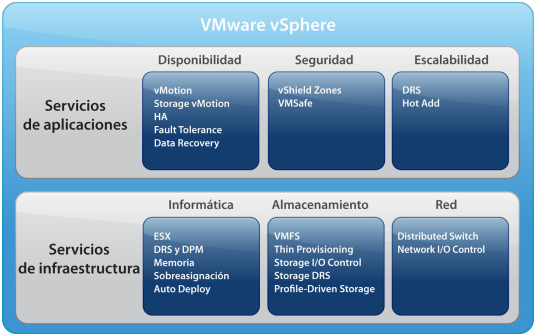
\includegraphics[width=0.75\textwidth]{imaxes/cap2recursos/contentVSphere}
  \caption{Elementos de la plataforma VMWare vSphere\cite{fotovSphere}}
  \label{fig:componentesVSphere}
\end{figure}
\begin{figure}[hp]
  \centering
  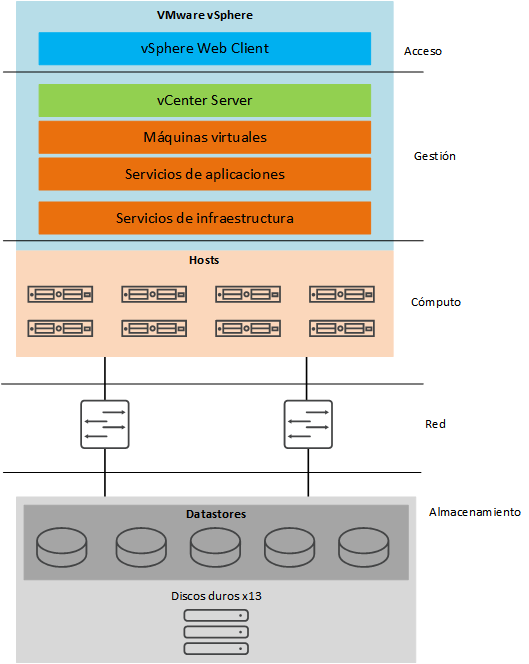
\includegraphics[width=1\textwidth]{imaxes/cap2recursos/recursosReal.png}
  \caption{Esquema de los recuros software y hardware del entorno}
  \label{fig:esquemaentornoreal}
\end{figure}

\FloatBarrier
\subsection{Estado de la tecnología}

En los últimos tiempos los servicios de \textit{Infrastructure as a Service} (IaaS) se han extendido de forma considerable con la aparición de software que permite la gestión de un sistema de Cloud Computing, como pueden ser VMware Cloud Foundation (2011), OpenStack (2010), o Apache CloudStack (2012). Estas herramientas construyen una infraestructura virtual sobre un entorno físico estandarizado que les permite administrar y automatizar la escalabilidad, el sistema de almacenamiento, la disponibilidad del servicio, la red, y la seguridad del servicio, con lo que se consigue reducir el coste y el tiempo de gestión y configuración, mejorando la eficiencia de infraestructura física.

A la hora de alcanzar los objetivos descritos en este proyecto se nos plantea la duda de que solución software desplegar ya que actualmente existen tres principales alternativas en el mercado, VMware Cloud Foundation, OpenStack y Apache CloudStack. Cada una de ellas ofrece diferentes características con diferentes requisitos que se pueden adaptar mejor o peor al entorno de despliegue, pero después de comprobar esos aspectos tenemos claro que la \underline{solución elegida es VMware Cloud Foundation}.

\subsubsection{VMware Cloud Foundation}
Esta solución virtualiza todas las capas de la infraestructura[Fig. \ref{fig:infraCloudFound}] (red, computación y almacenamiento) combinando cuatro componentes principales, vSphere para gestionar el cómputo, vSAN para la gestión del almacenamiento, NSX para la gestión de la red, y vRealize para gestionar todas las operaciones que tienen lugar en el servicio, integrando todos los componentes para que la gestión de la infraestructura sea lo más simple posible. Este cojunto de herramientas convierten el CPD en un \textit{Software Defined Datacenter} (SDDC), un entorno donde todas las partes físicas de la infraestructura pasan a estar controladas a través de software haciendo más flexible, independiente y menos costosa la configuración de estos componentes. Las \underline{principales características} de VMware Cloud Foundation son:
\begin{itemize}
    \item \textbf{Servicios software con integración nativa}: ofrece un conjunto de servicios software para el almacenamiento, red, seguridad y gestión de la cloud. Estos servicios se integran de forma nativa con la infraestructura minimizando las tareas de configuración y administración.
    \item \textbf{Escalabilidad y elasticidad de los recursos}: la capacidad de la infraestructura se puede modificar de forma sencilla gracias a la automatización del ciclo de vida de todos los elementos. 
    \item \textbf{Supervisión de los recursos}: ofrece supervisión de los recursos con reconocimiento de aplicaciones y solución de problemas, permitiendo conocer todos los eventos que tienen lugar en la infraestructura.
    \item \textbf{Aprovisionamiento automatizado}: todos los componentes necesarios para formar un SDDC son desplegados automáticamente por VMware Cloud Foundation, incluyendo los recursos informáticos, los componentes de almacenamiento, los de red y los de administración.
    \item \textbf{Ciclo de vida automatizado}: automatiza las operaciones previas, iniciales y posterios de una plataforma de software para ofrecer una gestión más sencilla. Esto incluye su implementación, el aprovisionamiento de clústeres aislados bajo demanda y la instalación de actualizaciones y parches.
   
   \iffalse 
    \item \textbf{Experiencia de usuario simple}: gracias a la gran cantidad de procesos automatizados.
    \item \textbf{Escalabilidad modular}: el sistema y la infraestructura se puede escalar de forma sencilla.
    \item \textbf{Cloud híbrida}: da la posibilidad de conectar una Cloud pública con una Cloud privada y así tratar ambas como una única Cloud.
    \fi
\end{itemize}

\begin{figure}[h!]
  \centering
  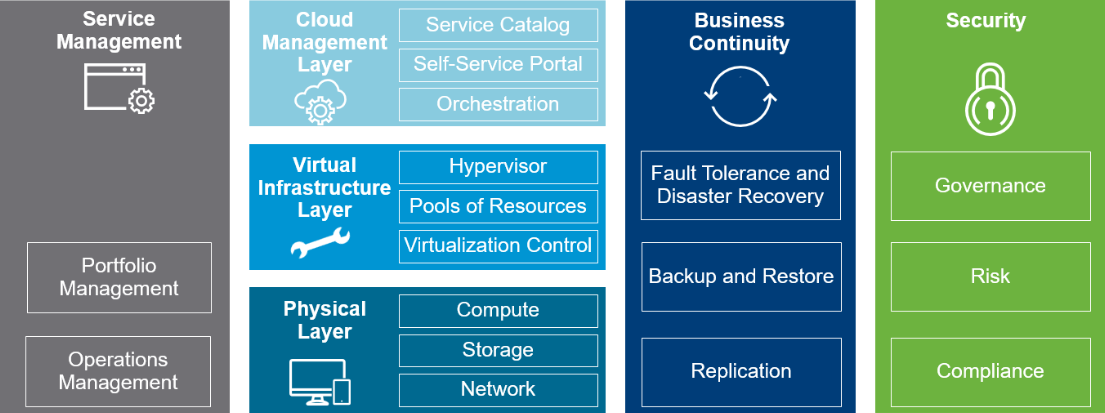
\includegraphics[width=1\textwidth]{imaxes/cap2recursos/SDDCoverview.png}
  \caption{Partes virtualizadas en un SDDC.}
  \label{fig:sddcoverview}
\end{figure}

\begin{figure}[h!]
  \centering
  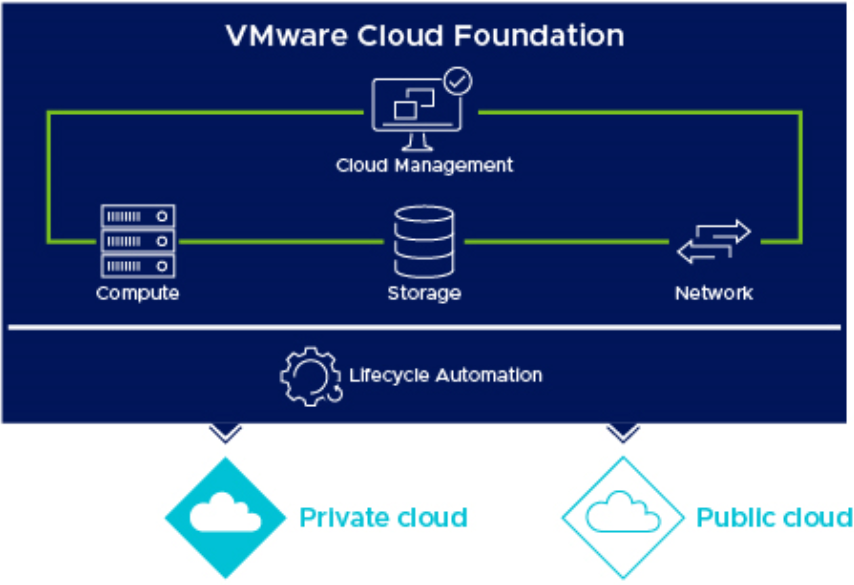
\includegraphics[width=1\textwidth]{imaxes/cap2recursos/overviewCF.png}
  \caption{Cloud Foundation virtualiza toda la infraestructura.}
  \label{fig:infraCloudFound}
\end{figure}
\FloatBarrier

VMware Cloud Foundation permite reducir el tiempo de mantenimiento ya que todo está controlado por el software que integra todos los componentes, automatizando gran parte de las operaciones y el ciclo de vida de todos los elementos desde su creación, como puede ser el control de versiones de cada elemento, los perfiles de usuario y las máquinas virtuales creadas, además de proporcionar una plataforma de acceso para que cada usuario pueda gestionar sus recursos. Además, su arquitectura se divide en entornos aislados administrados bajo demanda desde un entorno principal. Cada uno de esos entornos tiene un conjunto de recursos dedicados cuyas capacidades se pueden ajustar para proporcionar determinadas características, como por ejemplo alta disponibilidad, mayor capacidad de almacenamiento o mayor capacidad de cómputo. 

\iffalse
*****************************************************\\
También permite separar las cargas de trabajo mediante Dominios según el tipo de trabajo que se va a realizar, pudiendo acceder a cada uno de ellos de forma separada.\\
*****************************************************\\
\fi

Para poder usar este software es necesaria la adquisición de licencias, estas se organizan por componente y por número de hosts sobre los que se va a instalar el producto. A pesar de tener un coste elevado, teniendo en cuenta los beneficios que aporta en cuanto integración nativa con los componentes ya instalados y a que su mantenimiento es más sencillo, se ha elegido este paquete ya que es más rentable que otras opciones. \\
Si bien VMware ofrece plugins para conectar sus componentes con otras soluciones, como es el caso de OpenStack \cite{opestackintegrated}, estos no ofrecen el rendimiento que da la integración nativa, además, en caso de recibir actualizaciones, habría que actualizar cada componente de forma individual aumentando el riesgo de incompatibilidades con el resto de elementos del sistema, mientras que Cloud Foundation gestiona todo el ciclo de vida de cada actualización para cada componente, permitiendo comprobar si existe alguna incompatibilidad con el resto de versiones antes de aplicar una actualización. En definitiva, VmWare Cloud Foundation simplifica el proceso de instalación, configuración, gestión, y mantenimiento, tanto para los usuarios como para el administrador del sistema.

\subsubsection{Componentes de VMware Cloud Foundation \cite{componentesCloudFound}}
\label{subsubsect:cfcomponents}

\begin{figure}[h!]
  \centering
  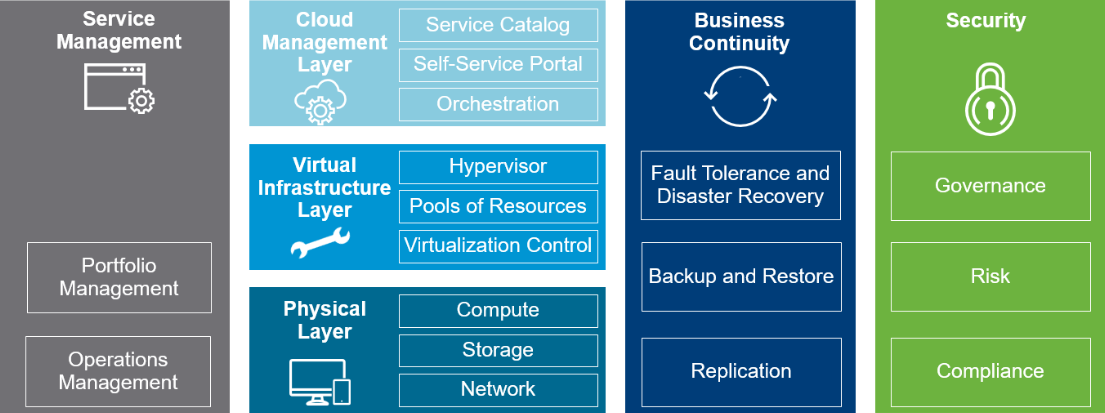
\includegraphics[width=1\textwidth]{imaxes/cap2recursos/SDDCoverview.png}
  \caption{Partes virtualizadas en un SDDC.}
  \label{fig:sddcoverview}
\end{figure}
\FloatBarrier

El SDDC de VMware Cloud Foundation está dividido en varias capas y módulos con las cuales se gestiona todas las partes de la infraestructura [Fig. \ref{fig:sddcoverview}]. Cada una de estas capas incluye una serie de productos y servicios, con unas funciones concretas que permiten gestionar un entorno complejo de una forma más sencilla. Las partes de esta infraestructura son las siguientes:
\begin{itemize}
    \item \textbf{Capa de Infraestructura física}: Es la base de la infraestructura y en ella residen los componentes físicos de almacenamiento, red y cómputo.
    \item \textbf{Capa de Infraestructura Virtual}: Se encuentra sobre la capa física y se encarga de realizar las tareas de acceso a los recursos físicos para controlar su aprovisionamiento.
    \item \textbf{Capa de Gestión Cloud}: Es la capa superior y se dedica a las tareas de consumo de los recursos, es decir, realiza peticiones a las capas inferiores para la obtención de los recursos.
    \item \textbf{Capa de Gestión de Servicios}: Esta capa se centra en el mantenimiento de la arquitectura gestionando el ciclo de vida, la monitorización, logs y alertas de los componentes. 
    \item \textbf{Capa de Gestión de Operaciones}: La función de esta capa es la monitorización de la capa de infraestructura física, de la capa de infraestructura virtual y de los flujos de trabajo de los usuarios.
    \item \textbf{Capa de Continuidad del Servicio}: Contiene elementos que ayudan a que el servicio se mantenga activo y a evitar la pérdida de información crítica, proveyendo copias de seguridad, restauración y recuperación ante desastres.
    \item \textbf{Capa de Seguridad}: Se encarga de que todos los componentes de la infraestructura estén bien delimitados para establecer un nivel de seguridad.
\end{itemize}

En VMware Cloud Foundation existen diversos productos y servicios, algunos son requeridos para construir la instancia mínima de un SDDC y otros ofrecen servicios adicionales que incrementan el rendimiento de la infraestructura. A continuación se describen aquellos componentes necesarios para la instalación mínima de VMware Cloud Foundation y que se usarán en la implementación de este proyecto:

\begin{itemize}
    \item \textbf{SDDC Manager}: gestiona el ciclo de vida de todos los componentes del sistema, incluyendo el proceso inicial de despliegue de Cloud Foundation, su configuración y aprovisionamiento, y las actualizaciones. Monitoriza los recursos físicos y lógicos de la infraestructura, facilita su configuración y permite añadir nuevos recursos cuando sea necesario. \iffalse Todo esto lo realiza mediante flujos de trabajo que facilitan la detección de orígenes de errores.\fi
    \item \textbf{vSphere}: ya está incluído en el servicio actual [\ref{subsec:softwareinstalado}].
    \item \textbf{VMware vSAN}: componente clave que virtualiza el almacenamiento. Como ya se ha explicado, el almacenamiento del servicio actual está configurado con LUNs que se deben gestionar individualmente en una capa distinta a los componentes software, provocando que su configuración sea más compleja y costosa. El objetivo de VMware vSAN es gestionar de forma automatizada y desde un único lugar el sistema de almacenamiento de la infraestructura, tratando toda la capacidad y recursos de almacenamiento como un único elemento, eliminando así la necesidad de tener que crear LUNs aisladas, consiguiendo abstraer la configuración de almacenamiento de la capa física en la capa de software y permitiendo establecer políticas de almacenamiento desde cada máquina virtual para adecuarlo a las necesidades de cada una sin tener que editar la configuración real del entorno físico. Así el rendimiento de los recursos de almacenamiento es más eficiente, flexible y su configuración se integra dentro del mismo servicio junto con la gestión del resto de componentes. \\
    En vSAN, en lugar de tratar el almacenamiento de forma independiente este pasa a estar ligado a cada host, es decir, cada uno de los nodos tiene asignados hasta cinco grupos de discos. Estos grupos de discos pueden ser \emp{Hybrid}, donde se combinan discos duros SSD y HDD, o \emp{All-Flash}, donde todos los discos utilizan tecnología \textit{Solid-State Drive} (SSD). Dentro de cada grupo hay \underline{dos tipos de discos} con distintas funciones, el disco de caché y el disco de capacidad\cite{operacionesVSAN}:
        \begin{itemize}
            \item \textbf{Caché}: Hay uno en cada grupo. Realiza la función de memoria caché y se encarga de escribir los datos persistentes en los discos de capacidad.
            \item \textbf{Capacidad}: Puede haber hasta siete discos en cada grupo. Almacena los datos persistentes del entorno.
        \end{itemize}
    En cada grupo de discos la gestión de la \underline{lectura y escritura} de datos se hace de la siguiente forma:
        \begin{itemize}
            \item \textbf{Lectura}: En el caso de la solución híbrida, si el dato que se busca no está en el disco de caché entonces se busca en los discos de capacidad y después se incorpora al disco de caché. Con la solución all-flash, los datos se leen siempre directamente de los discos de capacidad sin que estos sean escritos en el disco de caché dejando a este completamente libre para las operaciones de escritura. Gracias a esto, la estructura all-flash ofrece mayor rendimiento respecto a la híbrida.
            \item \textbf{Escritura}: Tanto en la solución híbrida con en la all-flash, el host ESXi primero escribe en el disco de caché, este le responde con una confirmación de escritura y más tarde vSAN se encarga de escribir ese dato en los discos de capacidad cuando el disco de caché está casi completo o cuando el dato lleva un tiempo sin ser utilizado.
        \end{itemize}
        \begin{figure}[h!]
            \centering
            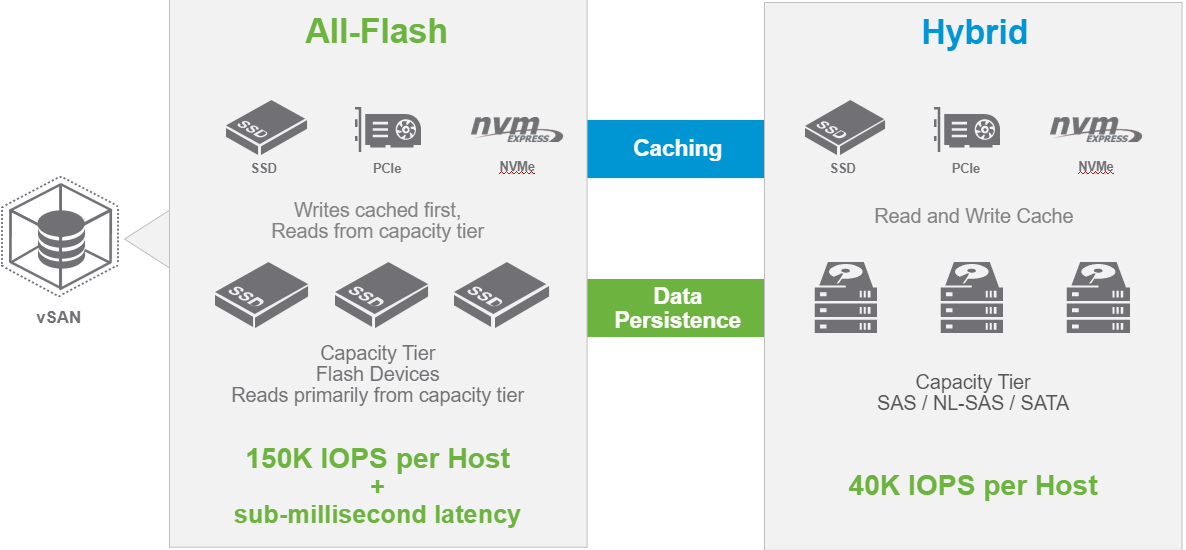
\includegraphics[width=1\textwidth]{imaxes/cap2recursos/rendimientoVSAN.png}
            \caption{Almacenamiento All-Flash vs. Híbrido en vSAN}
            \label{fig:rendimientoVSAN}
        \end{figure}
        \FloatBarrier
    Los hosts acceden al \textit{datastore} de vSAN mediante protocolo IP en una red accesible por todos los nodos. \\ 
    Este componente permite reducir las tareas de gestión del almacenamiento físico ya que ya no es necesario hacer ajustes en la capa física para cumplir unos requisitos en la capa software.
    \item \textbf{VMware NSX}: otro de los componentes clave. Tiene un papel similar a vSAN, pero en este caso se encarga de virtualización de los componentes físicos de la red de la infraestructura, es decir, abstrae los componentes físicos de nuestro entorno en software, dando más libertad a la hora de establecer la topología y componentes físicos de la red. Incluye servicios como firewall, elimina el tráfico  DNS, DHCP, VPN, NAT, enrutamiento, balanceo de carga, o switching, que permiten reducir la cantidad de dispositivos físicos de red.\\
    Principales \underline{componentes internos}\cite{componentesNSX}:
    \begin{itemize}
        \item \textbf{NSX Manager}: es el punto de entrada de la comunicaión con la instancia de vSphere, se encarga de desplegar NSX Controllers y el resto de servicios de NSX, instala VXLAN en los hosts ESXi, \textit{distributed routers} y firewalls, se comunica con los NSX Controllers y genera certificados para que las comunicaciones con los hosts ESXi sean seguras.
        \item \textbf{NSX Controller}: establece el punto de control desde donde se distribuye la información sobre el enrutamiento lógico y de VXLAN hacia los hosts ESXi, existen varios nodos de este tipo para facilitar el escalado y alta disponibilidad de la infraestructura, comparte la información de red entre el resto de NSX Controllers, abstrae el uso de VXLAN sobre la red física y elimina el uso del protocolo ARP en redes VXLAN. 
        \item \textbf{NSX Virtual Switch}: gestiona los vSphere vSwitch Distibuted desplegados, proporcionando switching entre los hosts ESXi.
        \item \textbf{NSX Logical Router Control}: se despliega cuando se crea un Distributed Logical Router. Se encarga de buscar adyacencias para generar tablas de enrutamiento que envía a NSX Manager y a los NSX Cotrollers para que informen a cada Distributed Logical Router en cada nodo ESXi.
        \item \textbf{NSX Edge}: proporciona servicios múltiples servicios como firewall perimetral de capa 2 y 3, SSL, NAT, DHCP, VPN, balanceo de carga y alta disponibilidad.
    \end{itemize}
    \item \textbf{VMware vRealize Log Insight}: realiza la gestión de logs del servicio, dando visibilidad a todas las operaciones del servicio, generando análisis del sistema. Esto permite tener mayor conocimiento de los riesgos, eficiencia y uso de recursos, a parte de facilitar la búsqueda de orígenes de errores.\\
    Forma un cluster que integra los siguientes \underline{componentes}:
    \begin{itemize}
        \item \textbf{Nodo Master}: cuando se despliega con el modo \textit{standalone} este el responsable de todas las actividades, incluyendo las consultas de los clientes para obtener los logs y las tareas de obtención de los logs. Este nodo se encarga de las operaciones del cluster que forman los nodos de VMware Realize Log Insight como actualizaciones, creación y eliminación de nodos, tanto en modo \textit{standalone} como en entornos de alta disponibilidad. 
        
        \item \textbf{Nodo Worker}: es un nodo opcional que se crea para proporcionar alta disponibilidad y escalar el entorno, facilitando la escalabilidad del entorno. En estos nodos se delegan la gestión de las consultas de los clientes y de la obtención de logs que el nodo \textit{master} realiza en el modo \textit{standalone}.
        \item \textbf{Load Balancer}: se encarga de centralizar y asegurar la entrada de logs en VMware vRealize Log Insight simplificando la creación de nodos a medida que se van creando. Además, se encarga del balancear el tráfico entrante entre todos los nodos y de escoger el nodo \textit{master}. Se ejecuta en uno de los nodos del cluster.
    \end{itemize}
    
    \item \textbf{VMware vRealize Automation}: se trata de un componente opcional que permite automatizar el despliegue de máquinas virtuales, procesos y aplicaciones reduciendo la complejidad y eliminando tareas manuales. Esto acelera la entrega del servicio gracias a que las tareas de aprovisionamiento y entrega de recursos y aplicaciones son más rápidas permitiendo establecer políticas de seguridad y control. Internamente, este servicio \underline{cuenta con los siguientes componentes \cite{vRealizeAutomation}} para cumplir con sus funciones:
    \begin{itemize}
        \item \textbf{vRealize Automation Appliance}: contiene un portal donde los usuarios pueden acceder y gestionar y aprovisionar servicios cloud bajo demanda, un servicio de autenticación y una interfaz para gestionar este componente. 
        \item \textbf{IaaS Web Server}: realiza las tareas de administración de la infraestructura que se requieren desde el portal de vRealize Automation Appliance.
        \item \textbf{Microsoft SQL Server}: se utiliza para almacenar información sobre los elementos de IaaS y sobre las máquinas virtuales controladas por vRealize Automation Appliance.
    \end{itemize}
\end{itemize}

**Decir como se puede implementar un sistema de facturación.*******\\
**Como se puede conectar los usuarios de la UDC.********












\iffalse
\subsubsection{OpenStack}
Es una plataforma constituída por tres proyectos, uno dedicado a la gestión de la red, otro a la gestión del cómputo, y otro a la gestión del almacenamiento. Para poder desplegarlo sobre los componentes de VmWare instalados en nuestra infraestructura son necesarios tres plugins específicos para el software de VmWare. OpenStack aporta una API a través de la cual es posible gestionar los recursos virtuales y el aproivisionamiento.

\subsubsection{Apache CloudStack}
\fi



 \begin{chapter}{Planificación}
\label{chap:planificacionProyecto}
\lettrine{E}{n} este capítulo se propone una planificación del proyecto con el fin de organizar su estructura y exponer sus costes temporales y económicos aproximados necesarios para su realización.
\begin{section}{Tareas y costes del proyecto}
\underline{Tarea 1}. Analizar qué componentes hardware y software componen la infraestructura y cuales son sus funciones. En cuanto al hardware se comprueban las especificaciones concretas de los recursos de cómputo, almacenamiento y red, y cómo están estructurados el sistema de almacenamiento y la red. Respecto al software se comprueba qué productos y servicios hay instalados y cuales son sus funciones dentro del entorno.\\
% \underline{Tarea 1}. Analizar como está formada la infraestructura, que componentes hardware y software la componen y cual es la función de cada uno de ellos. En cuanto a la parte física se comprueban las especificaciones concretas del hardware de cómputo, almacenamiento y red. También como están organizados y estructurados tanto el sistema de almacenamiento y la red de la infraestructura. En la parte de software, se detallan las funciones de los principales programas y servicios que están instalados en el entorno.\\
\underline{Tarea 2}. Analizar y seleccionar una herramienta de las disponibles en el mercado que se adapte a los objetivos del servicio que se quiere construir y a las características de la infraestructura. En este proceso se tiene en cuenta la compatibilidad con el software ya existente, el coste de mantenimiento y la eficiencia de las herramientas disponibles.\\
\underline{Tarea 3}. Tarea que agrupa las tareas dedicadas al proceso de configuración de la infraestructura e instalación y configuración de la herramienta seleccionada. Estas son las tareas 4, 5, 6, 7, 8, 9 y 10.\\
\underline{Tareas 4, 5, 6, 7, 8, 9 y 10.} Antes de realizar la instalación de la nueva herramienta es necesario comprobar sus requisitos software y hardware (tareas 4 y 5). También se deben establecer los parámetros de configuración iniciales que se van a aplicar a la nueva plataforma (tarea 6). Construcción de un entorno de pruebas con una infraestructura que se adapte a los requisitos de la herramienta seleccionada y así evitar problemas en el entorno real del CITIC (tareas 7 y 8). Una vez el entorno está preparado se efectúa el despliegue de la herramienta(tarea 9), posteriormente se configura y se comprueba el funcionamiento del nuevo servicio (tarea 10).\\
% \underline{Tareas 4, 5, 6, 7, 8, 9 y 10.} Con el objetivo de desplegar la herramienta seleccionada anteriormente se llevan a cabo las siguientes tareasComprobación de requisitos, preparación del entorno, establecimiento de parámetros configuración, despliegue de la plataforma sobre la infraestructura existente y configuración de la plataforma después del despliegue. Antes de realizar la instalación de la nueva herramienta es necesario comprobar sus requisitos necesarios para que las capacidades del servicio final se adapten a las necesidades de uso (tareas 4 y 5). También se deben establecer los parámetros de configuración iniciales que se van a aplicar a la nueva plataforma (tarea 6). Durante el proceso de comprobación de requisitos puede surgir la necesidad de realizar cambios sobre las capacidades de la infraestructura y la configuración de los componentes ya existentes en el entorno inicial para que este se adapte a los requisitos de la nueva plataforma (tareas 7 y 8). Una vez el entorno está preparado para la herramienta pueda ser instalada entonces se efectúa el despliegue (tarea 9), posteriormente se configura y se comprueba el funcionamiento del nuevo servicio (tarea 10).\\
\underline{Tarea 11.} Esta tarea marca el final del despliegue y configuración del nuevo servicio en la infraestructura.\\
\underline{Tarea 12}. Diseñar una integración de la nueva plataforma con el sistema de autenticación de la UDC para que los usuarios finales del servicio puedan autenticarse sin necesitar nuevas credenciales. Se debe utilizar un directorio de usuarios que simule el directorio de la UDC y así evitar problemas en el entorno de producción.\\
% \underline{Tarea 12}. Diseñar una integración de la nueva plataforma con el sistema de autenticación de la UDC para que los usuarios finales del servicio puedan autenticarse sin necesitar nuevas credenciales. Para ello es preciso comprobar el método de acceso al directorio de usuarios de la UDC y la forma de conectarlo con la plataforma desplegada para, posteriormente, realizar un diseño de la solución. Este proceso requiere realizar una solicitud de acceso a los servicios internos de la UDC.\\
\underline{Tarea 13}. Implementación y despliegue de la solución que permita integrar el directorio de usuarios del entorno de pruebas con la herramienta desplegada para la autenticación de usuarios con sus propias credenciales.\\
% \underline{Tarea 14}. Análisis del uso que harán los usuarios del servicio para establecer políticas sobre el uso de recursos. Para realizar este cálculo, primero se debe analizar el uso previo al despliegue del nuevo servicio que los usuarios hacen de la infraestructura y, después, estimar el uso que pueden llegar a realizar una vez el servicio sea accesible. Hay que tener en cuenta la cantidad de usuarios que lo utilizan, que lo van a utilizar y la cantidad de recursos que se emplean y que se van a emplear. Una vez obtenida una estimación, se realiza un diseño de las políticas que se van a aplicar.\\
\underline{Tarea 14}. Diseño de un sistema de facturación/valoración del consumo de recursos por parte de los usuarios con la intención de limitar la cantidad de recursos que un usuario puede aprovisionar, y así tener recursos disponibles para todos los usuarios y aumentar la eficiencia la eficiencia de la infraestructura.\\
% \underline{Tarea 15}. Diseño de un sistema de facturación/valoración de los recursos del servicio en base a las políticas de uso establecidas. Basándose en las políticas establecidas en la tarea 14, se debe pensar como se pueden aplicar sobre el servicio. Esto puede ser a través de una herramienta externa, en ese caso sería necesario realizar un desarrollo, o integrando la configuración en los parámetros de configuración de la plataforma.\\
% La intención de este sistema es limitar la cantidad de recursos que un usuario puede aprovisionar permitiendo aumentar la eficiencia de los recursos físicos reduciendo la cantidad de recursos ociosos.\\
\underline{Tarea 15}. Implementación y despliegue del sistema de facturación/valoración.\\
% \underline{Tarea 16}. Implementación y despliegue del sistema de facturación/valoración. Para implementar este sistema puede que sea necesario realizar el desarrollo de una herramienta si se determina que no es posible establecerlo a través de los parámetros de configuración de la plataforma. \\
\underline{Tarea 16, 17 y 18}. Recopilación de la información necesaria para la realización de cada tarea. La información de apoyo se debe obtener de documentaciones, artículos, vídeos o libros de  fuentes fiables como empresas desarrolladoras de los productos utilizados o expertos especializados. El objetivo la recopilación de información es obtener conocimiento sobre las herramientas con las que se está trabajando para luego tener una base que facilite la realización de las tareas descritas. Esto se realiza desde el comienzo del proyecto hasta su finalización para tener claros los conceptos que se desarrollan y para conocer los detalles del trabajo que se realiza.\\
\underline{Tarea 19, 20 y 21}. Redacción de la memoria del proyecto. Se escribe un documento con todos los detalles de todas las tareas realizadas durante el proyecto, incluyendo los cambios realizados en la infraestructura, las configuraciones establecidas y como se lleva a cabo cada proceso del proyecto. Su objetivo es transmitir el conocimiento adquirido durante su realización y proponer una solución para habilitar un servicio Cloud en la infraestructura del CITIC. La escritura de este documento se realiza a la vez que cada tarea para detallar los pasos realizados en cada caso, por lo que su duración es igual a la duración total de todo el proyecto.\\
% \underline{Tarea 20, 21 y 22}. Redacción de la memoria del proyecto. Se escribe un documento con todos los detalles de todas las tareas realizadas durante el proyecto, incluyendo los cambios realizados en la infraestructura, las configuraciones establecidas y como se lleva a cabo cada proceso del proyecto. Su objetivo es transmitir el conocimiento adquirido durante el proyecto sobre como realizar el despliegue de una plataforma de virtualización y los beneficios que esta puede tener. La escritura de este documento se realiza a la vez que completa cada tarea para detallar los pasos realizados en cada caso, por lo que su duración es igual a la duración total de todo el proyecto.\\

La duración total del proyecto se estima en 101 días. teniendo en cuenta que el estudiante trabaja durante 4 horas diarias. El coste mostrado en la figura \ref{fig:estadisticasproyecto} se refiere al coste correspondiente al estudiante si trabaja por 25 €/hora. 
\begin{figure}[h!]
  \centering
  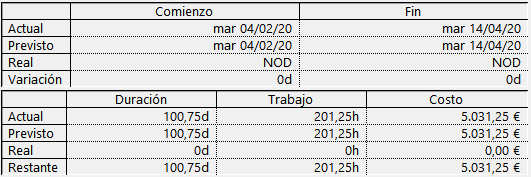
\includegraphics[width=1\textwidth]{imaxes/extras/estadisticasProyecto.png}
  \caption{Estadísticas sobre la planificación del proyecto.}
  \label{fig:estadisticasproyecto}
\end{figure}
\FloatBarrier
\begin{landscape}
\begin{figure}[hp]
  \centering
  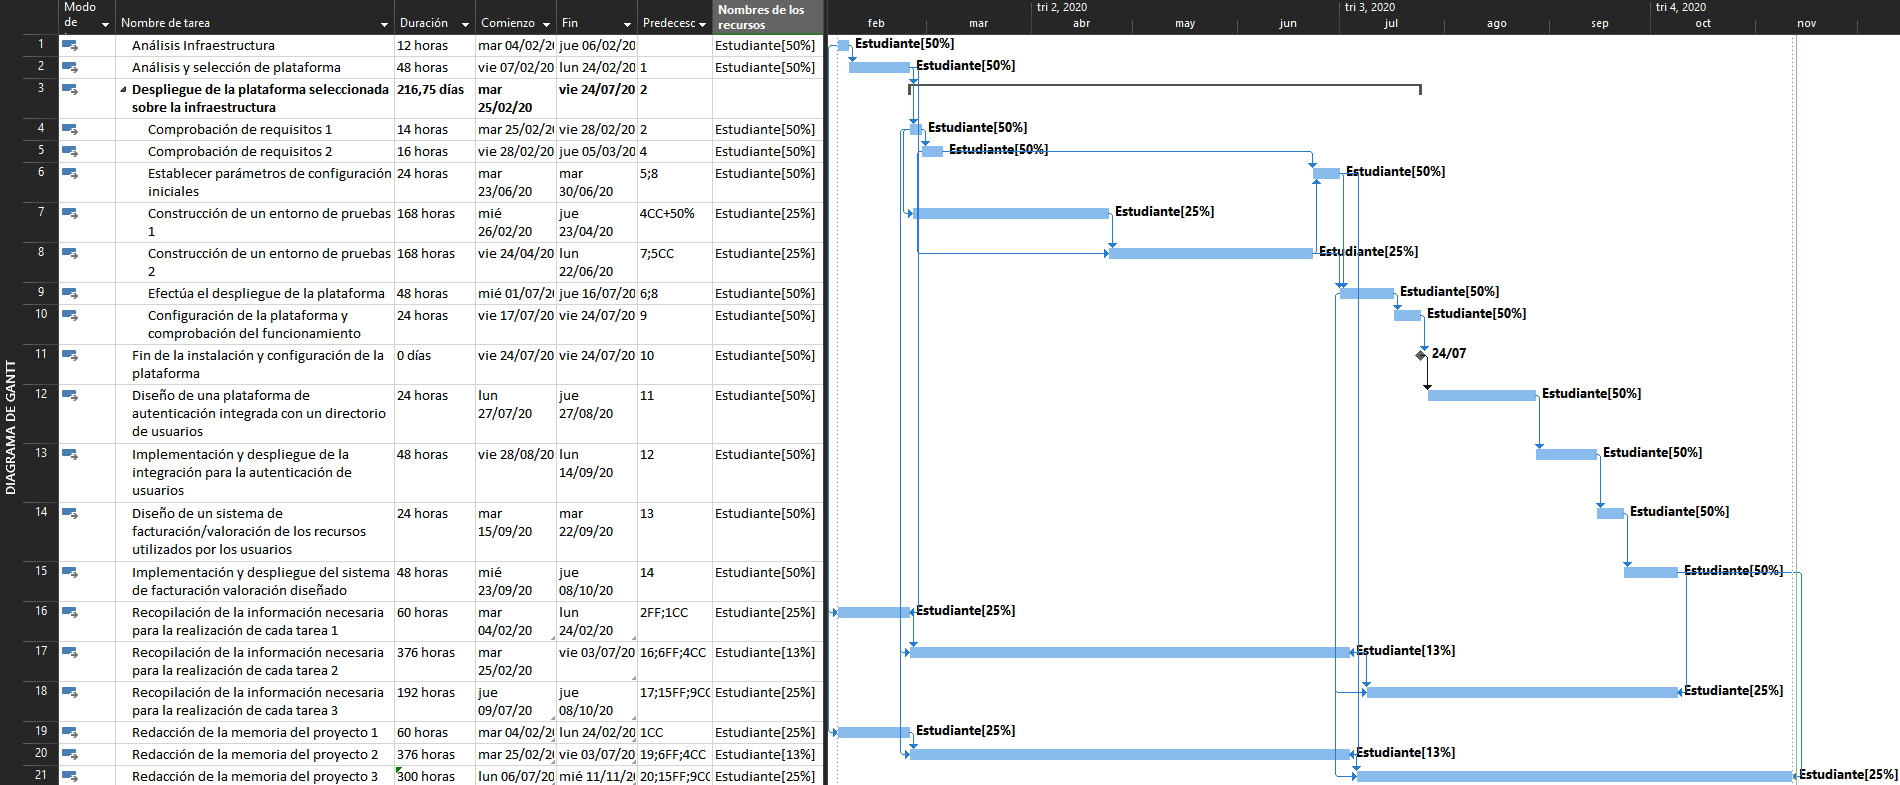
\includegraphics[width=1.5\textwidth]{imaxes/extras/diagramaGranttt.png}
  \caption{Diagrama de Grantt sobre la planificación del proyecto.}
  \label{fig:tareasproyecto}
\end{figure}
\end{landscape}
\FloatBarrier
\end{section}

% \begin{section}{Costes de implementación}
% Los principales costes de implementar la solución propuesta en la infraestructura de producción del CITIC son aquellos relacionados con los trabajadores que lo llevan a cabo y las licencias necesarias para cada componente de VMware Cloud Foundation\footnote{Los componentes que se especifican son aquellos que son obligatorios para desplegar VMware Cloud Foundation.}.\\
% Cada componente de VMware Cloud Foundation requiere su propia licencia\cite{licenses}. El precio de cada licencia dependerá del número de CPUs físicas sobre las que se va usar esta plataforma por lo que, como en la infraestructura hay un total de ocho hosts con dos CPUs cada uno, \underline{el precio por cada componente} es el siguiente:
% \begin{itemize}
%     \item \textbf{SDDC Manager}: 18.000€\footnote{Para la edición \textit{Advanced} de VMware Cloud Foundation.} por CPU y 6.500€ anuales de soporte por cada CPU. El precio total de la licencia es de 288.000€ y 104.000€ anuales de soporte por 16 CPUs.
%     \item \textbf{VMware vSphere}: 4.000€\footnote{Para la edición \textit{Standard} de VMware vSphere.} por CPU. El precio total de la licencia es de 64.000€ por 16 CPUs y el precio anual por las tareas de soporte es de 16.000€.
%     \item \textbf{VMware vCenter}: 6.000€\footnote{Para la edición \textit{Standard} de VMware vCenter} por una licencia que permite usar VMware vCenter sobre todos los hosts del entorno. El precio anual por las tareas de soporte es de 1.500€.
%     \item \textbf{VMware vSAN}: 4.000€\footnote{Para la edición \textit{Advanced} de VMware vSAN.} por CPU. El precio total de la licencia es de 64.000€ por 16 CPUs y el precio anual por las tareas de soporte es de 16.000€.
%     \item \textbf{VMware NSX-T}: 5.300€\footnote{Para la edición \textit{Advanced} de NSX.} por CPU. El precio total de la licencia es de 84.400€ por 16 CPUs y el precio anual por las tareas de soporte es de 21.100€.
%     \item \textbf{VMware vRealize Suite 2019}: 1.500€ por CPU. El precio total de la licencia es de 24.000€ por 16 CPUs y el precio anual por las tareas de soporte es de 6.000€.
% \end{itemize}

% El precio total de todas las licencias necesarias para el entorno, teniendo en cuenta que hay 16 CPUs, sería igual a 530.400€, y el precio total por las tareas de soporte sería igual a 164.600€ anuales.\\

% En caso de que ya estén instalados algunos de los componentes entonces solo se requieren licencias para aquellos componentes que aún no están en el entorno. En el caso del entorno inicial, los componentes que ya están instalados son VMware vSphere, VMware vCenter Server. Esto hace que el \underline{coste real para implementar VMware Cloud Foundation} en el entorno sea igual a 460.400€, ya que solo son necesarias licencias para los componentes SDDC Manager, VMware vSAN, VMware NSX-T y VMware vRealize Suite 2019. El coste total de la instalación y mantenimiento de la plataforma VMware Cloud Foundation sobre la infraestructura del CITIC es el siguiente:

%     \begin{itemize}
%         \item \textbf{Licencias}: 460.400€ en total.
%         \item \textbf{Soporte}: 164.600€ anuales.
%         \item \textbf{Sueldo empleado}: 5.031,25€ en total.
%     \end{itemize}
%   \end{section}

  \end{chapter}
 %\chapter{Metodología}
\label{chap:demo}


\lettrine{E}{ntre} a introdución e as conclusións, o documento conterá
tantos capítulos como sexa preciso, sempre con coidado de non rebasar
o límite de 80 páxinas fixado polo regulamento de TFGs.

Empregaremos éste de xeito demostrativo, para ilustrar o uso de
elementos habituais que poidan ser de utilidade.

\section{Inclusión de imaxes}

Se precisamos imaxes no noso documento, incluirémolas do xeito que se
indica na figura~\ref{fig:exemplo} (páxina~\pageref{fig:exemplo}). Se
o facemos así, \LaTeX ubicará cada imaxe no mellor lugar posible,
lugar que pode variar a medida que o documento vaia crecendo coa
inclusión de máis texto e outros elementos (máis imaxes, táboas,
etc.).

\begin{figure}[hp!]
  \centering
  
\includegraphics[width=0.75\textwidth]{imaxes/udc.png}
  \caption{Pé de imaxe descritivo}
  \label{fig:exemplo}
\end{figure}

Recoméndase almacenar os ficheiros gráficos no directorio
\texttt{imaxes}.

\subsection{Inclusión de varias sub-imaxes}

Se precisamos inserir imaxes relacionadas, pode ser apropiado
incluílas como sub-figuras, do xeito que se pode apreciar na
figura~\ref{fig:exemplo-subfiguras} coas
imaxes~\ref{fig:subfigura-rotada}
e~\ref{fig:subfigura-deformada}. Como se pode ver nos exemplos desta
sección, sempre é recomendable referirse ás imaxes pola súa
referencia, xa que dese xeito non dependemos de onde queden ubicados
os elementos en cuestión.

\begin{figure}[hp!]
  \centering
  \begin{subfigure}[c]{0.3\textwidth}
    
\includegraphics[angle=45,width=\textwidth]{imaxes/udc.png}
    \caption{Pé de subimaxe rotada}
    \label{fig:subfigura-rotada}
  \end{subfigure}
  \hspace{0.1\textwidth}
  \begin{subfigure}[c]{0.3\textwidth}
    
\includegraphics[width=\textwidth,height=3cm]{imaxes/udc.png}
    \caption{Pé de subimaxe deformada}
    \label{fig:subfigura-deformada}
  \end{subfigure}
  \caption{Pé de imaxe xeral}
  \label{fig:exemplo-subfiguras}
\end{figure}

\section{Inclusión de código fonte}

Se precisamos incluír fragmentos de código fonte, podemos facelo da
seguinte maneira:

\begin{lstlisting}[language=C]
#include <stdio.h>
#define N 10

int main()
{
  int i;

  // Isto é un comentario
  puts("Ola, mundo!");

  for (i = 0; i < N; i++)
  {
    puts("LaTeX é a ferramenta de edición ideal para profesionais da informática!");
  }

  return 0;
}
\end{lstlisting}

%\include{contido/...}
 \chapter{Conclusións}
\label{chap:conclusions}

\lettrine{D}{erradeiro} capítulo da memoria, onde se presentará a
situación final do traballo, as leccións aprendidas, a relación coas
competencias da titulación en xeral e a mención en particular,
posibles liñas futuras,\dots

\Blindtext


 %%%%%%%%%%%%%%%%%%%%%%%%%%%%%%%%%%%%%%%%
 % Apéndices, glosarios e bibliografía  %
 %%%%%%%%%%%%%%%%%%%%%%%%%%%%%%%%%%%%%%%%

 \appendix
 \appendixpage
 \chapter{Material adicional}
\label{chap:adicional}

Shell script para la limpieza de una máquina virtual Ubuntu después de haber configurado cloud-init. Obtenido del siguiente repositorio \url{https://github.com/jimangel/ubuntu-18.04-scripts}.
\lstinputlisting[language=bash]{anexos/file/clean-ubuntu.sh}

%\include{anexos/...}

 \chapter*{\nomeglosarioacronimos}
\addcontentsline{toc}{chapter}{\nomeglosarioacronimos}
\label{chap:acronimos}

%%%%%%%%%%%%%%%%%%%%%%%%%%%%%%%%%%%%%%%%%%%%%%%%%%%%%%%%%%%%%%%%%%%%%%%%%%%%%%%%
% Obxectivo: Lista de siglas, abreviaturas, acrónimos, etc. empregados         %
%            no documento, xunto cos seus respectivos significados.            %
%%%%%%%%%%%%%%%%%%%%%%%%%%%%%%%%%%%%%%%%%%%%%%%%%%%%%%%%%%%%%%%%%%%%%%%%%%%%%%%%

\begin{description}
 \item [ERLANG/OTP] \emph{Erlang Open Telecom Platform}.
\end{description}

%%%%%%%%%%%%%%%%%%%%%%%%%%%%%%%%%%%%%%%%%%%%%%%%%%%%%%%%%%%%%%%%%%%%%%%%%%%%%%%%

 \chapter*{\nomeglosariotermos}
\addcontentsline{toc}{chapter}{\nomeglosariotermos}
\label{chap:glosario-termos}

%%%%%%%%%%%%%%%%%%%%%%%%%%%%%%%%%%%%%%%%%%%%%%%%%%%%%%%%%%%%%%%%%%%%%%%%%%%%%%%%
% Obxectivo: Lista de termos empregados no documento,                          %
%            xunto cos seus respectivos significados.                          %
%%%%%%%%%%%%%%%%%%%%%%%%%%%%%%%%%%%%%%%%%%%%%%%%%%%%%%%%%%%%%%%%%%%%%%%%%%%%%%%%

\begin{description}
 \item [Tenencia múltiple]: principio de la arquitectura de software donde una aplicación se sirve a varios clientes desde una misma instancia.
 \label{itm:tenenciamultiple}
 \item [SDDC]: \textit{Software Defined DataCenter} es un modelo de infraestructura donde se virtualiza la abstracción, gestión y automatización de todos los recursos y servicios de un centro de datos.
 \item [Hipervisor baremetal]: software instalado sobre el hardware de un servidor que permite instalar aplicaciones que funcionan sobre entornos virtuales directamente sobre el hardware.
  \label{itm:baremetal}
 \item [Máquina virtual]: software que emula un conjunto de recursos físicos para ejecutar otro software de forma aislada.
  \label{itm:vm}
 \item [Datastore]: contenedores que VMware vSphere utiliza para el almacenamiento archivos en un único lugar o a través de una red. Suelen utilizarse para almacenar ficheros de máquinas virtuales y puedent tener el formato VMFS, NFS o NAS.
 \label{itm:datastore}
 \item [Modelo multi-tenant]: es un modelo de desarrollo donde una misma aplicación se entrega a distintos usuarios sin hacer un desarrollo específico para cada uno de ellos.
 \label{itm:multitenant}
 \item [RAID 5]: Es un conjunto de discos duros que funciona como una única unidad de almacenamiento para aumentar el rendimiento y la eficiencia. RAID 5 necesita como mínimo tres discos duros, y distribuye la información de paridad en todos los discos (esta información permite recuperar datos corruptos a partir del resto de información no perdida).
 \label{itm:raid5}
 \item [Almacén de datos]
 \label{itm:almacendatos}
 \item [LUN]: \textit{Logical Unit Number} es un identificador que agrupa un agrupa un conjunto o subconjunto de almacenamiento físico o virtual. Puede asignarse a un disco completo o solo a una parte.
 \label{itm:lun}
 \item [Controlador SFP+]: módulo transceptor óptico que se utiliza en las telecomunicaciones y aplicaciones de transmisión de datos. Soportan Sonet, canal de Fibra y Gigabit Ethernet.
 \label{itm:sfp}
 \item [SAN]: \textit{Storage Area Network} es una red dedicada al almacenamiento, de alta velocidad con canal de Fibra o iSCSI, con equipos de conexión dedicados (p.e. switches) y con dispositivos de almacenamiento (discos duros). 
 \label{itm:san}
 \item [VMFS]: sistema de archivos de alto rendimiento nativo de VMware vSphere. Se utiliza para implementar los almacenes de datos y está optimizado para el almacenamiento de máquinas virtuales.
 \label{itm:vmfs}
 \item [Platform Services Controller (PSC)]: componente de la infraestructura que agrupa los servicios de infraestructura de un entorno vSphere. Estos servicios son la concesión de licencias, administración de certificados y la autenticación con vCenter Single Sign-On.
 \label{itm:psc}
 \item [Cluster]: Conjunto de dos o más Hosts para aprovisionar recursos.
 \label{itm:cluster}
 \item [Servicio LBT]: servicio que se encarga de balancear el tráfico que entra en cada interfaz de un switch.
 \item [vCPU]
 \label{itm:vcpu}
 \item [Jumbo Frame]: son los paquetes que se transmiten por una red y cuyo MTU es mayor a 1500.
 \label{itm:jumboframe}
 \item [VTEP]: \textit{VXLAN Tunnel End Point} es un componente del protocolo VXLAN cuya función es encapsular y desencapsular las tramas correspondientes a una VXLAN. Este componente se encuentra al principio y al final del camino que sigue una trama.
 \label{itm:vtep}
 \item [NIC]: \textit{Network Interface Controller} es un componente físico que conecta el host con una red.
 \label{itm:nic}
\end{description}


 %\bibliographystyle{IEEEtran}
 %\bibliography{\bibconfig,bibliografia/bibliografia}
 \cleardoublepage
 
\end{document}

%%%%%%%%%%%%%%%%%%%%%%%%%%%%%%%%%%%%%%%%%%%%%%%%%%%%%%%%%%%%%%%%%%%%%%%%%%%%%%%%
